Die Studie wurde im Rahmen des Verbundprojektes BACOSA (Baltic Coastal System Analysis and Status Evaluation) durchgeführt, bei dem in Zusammenarbeit der Universitäten Kiel, Rostock und Greifswald die Flachgewässer der südlichen deutschen Ostsee untersucht werden. Die Studie umfasst den Zeitrahmen April 2013 bis April 2016 und setzt sich zum Ziel, die Funktionen der Ökosysteme ausgewählter Buchten der Ostsee in einer möglichst umfassenden Gesamtheit zu verstehen, insbesondere die Auswirkung von Makrophyten auf die Sedimentdynamik und die Erfassung der Pelagial-Benthos-Wechselwirkung hinsichtlich der Stofftransporte. Außerdem werden auf Basis vorhandener Daten die Ökosystemdienstleistungen dieser Gewässer bewertet. Die Forschungsergebnisse sollen zum grundsätzlichen Verständnis der Ökosysteme beitragen und damit eine Grundlage zum Erfüllen der Forderungen der Europäischen Meeresstrategierichtlinie (EU-MSRL) und der Europäischen Wasserrahmenrichtlinie (EU-WRRL) schaffen. In dieser Diplomarbeit werden die Wechselwirkungen von Makrophyten und Sedimentstruktur charakterisiert.

Es ist allgemein bekannt, dass es Interaktionen zwischen dem Makrophytenbewuchs, der Hydrodynamik und der Sedimentdynamik in Süßwasser- und in marinen Systemen gibt. In vielen Studien im Freiland und in Strömungskanälen wurde festgestellt, dass dichte Makrophytenbestände dazu in der Lage sind das Strömungsregime so zu beeinflussen, dass die Sedimentation gefördert und die Resuspension vermindert wird. Wenn sich dies auch in Freilandversuchen in Buchten und Boddengewässern der Ostsee bestätigen ließe, ergäbe sich hieraus eine wichtige Funktion der Makrophytenbetten als lokale Nährstoffsenke und ein wichtiger Ansatz zum Verständnis von Stoffflüssen im Zuge der Gewässereutrophierung. In diesem Zusammenhang trägt die Arbeit dazu bei herauszufinden, welche vorhandenen Makrophytenbestände in welcher Intensität, unter welchen lokalen Strömungsbedingungen und in welchem Maß die Funktion als lokale Nährstoffsenke erfüllen.

Die Interaktionen zwischen den Faktoren Pflanzenwuchs, Strömung und Sediment sind sehr komplex. Pflanzen haben einen Einfluss auf die Strömung, indem sie Schwingungen mit niedriger Frequenz (Large Scale Eddies) zu Schwingungen mit hoher Frequenz (Small Scale Eddies) umbrechen und damit Turbulenzen verursachen \citep{leonard_2006}. Außerdem wird die Strömungsgeschwindigkeit innerhalb eines Pflanzenbestandes mit zunehmenden Deckungsgraden herabsetzt, während sie überhalb des Kronendaches unverändert hoch bleibt \citep{li_2014}.

Die Strömungsgeschwindigkeit hat umgekehrt auch einen Einfluss auf das Makrophytenwachstum. So können starke Strömungen und Wellenschlag die Pflanzen mechanisch schädigen und wachstumsreduzierend wirken \citep{biggs_1996}. Myriophyllum spicatum profitiert hiervon wiederum weil abgerissene Sprossteile wurzeln können und auf diese Art eine vegetative Vermehrung stattfindet \citep{madsen_1997}. Bei geringen Strömungen von \unit{0 bis 0,1}{\metre\per\second} hingegen wirkt sich eine leicht erhöhte Strömungsgeschwindigkeit positiv auf Wachstum und Photosyntheserate der Pflanzen aus \citep{madsen_1983}.

Die Strömung wiederum ist ein wichtiger Parameter für die Korngrößenverteilung des Sedimentes, da sie die Scherkraft und damit die Bodenschubspannung auf eine bestimmte Fläche des Seebodens positiv beeinflusst. Wird die für ein Korn kritische bodennahe Strömungsgeschwindigkeit (friction velocity) überschritten, gerät es in Bewegung, löst sich unter Überwindung von Schwerkraft und Partikelanziehung aus dem Sediment (Erosion) und wird in der Wassersäule gelöst (Resuspension) \citep{madsen_2001}. Nach Studien mit Seesedimenten im Strömungskanal von \cite{hu_2011} erhöht sich die Resuspension mit steigender Strömungsgeschwindigkeit. 
Der direkte Zusammenhang der gesteigerten Resuspension und der erhöhten Sedimentation in Makrophytenbetten gegenüber vegetationsfreien Flächen wurde in zahlreichen limnischen Freilandstudien \citep{horppila_2003, horppila_2005}, und auch in Buchten der Ostsee \citep{kaitaranta_2013} bei einem Anteil von Makrophyten in der Wasserfläche von \unit{30 bis 35}{\%}, gefunden.

\cite{ward_1984} sowie \cite{fonseca_1986} fanden zudem einen Unterschied hinsichtlich der Resuspension bei unterschiedllichen Anteilen der Pflanzen an der Wassersäule. Die Strömungsgeschwindigkeiten wurden umso effizienter reduziert und das Material umso mehr akkumuliert, je höher der Anteil der Makrophyten an der Wassersäle war. Es ist nach \cite{madsen_2001} davon auszugehen, dass sich die Makrophyten durch ihre Anwesenheit einen positiven Feedbackloop verschaffen, indem sie durch Steigerung der Sedimentation und die Reduzierung der Resuspension die Trübung vermindern und damit die Lichtverfügbarkeit am Grund zum Vorteil der eigenen Photosyntheseleistung erhöhen.

In Makrophytenbetten befindet sich nach \cite{kenworthy_1982} auch mehr organisches Material im Sediment als im makrophytenfreiem Bereich. Erst bei starken Windereignissen kann es hier zu schlagartigen Resuspensionsereignissen kommen, bei denen das feine organische Material und damit Nährstoffe in die Wassersäule gelangen \citep{dauby_1995}. Hierdurch wird das Phytoplanktonwachstum angekurbelt \citep{cowan_1996}.

\begin{figure}[htb]
\centering
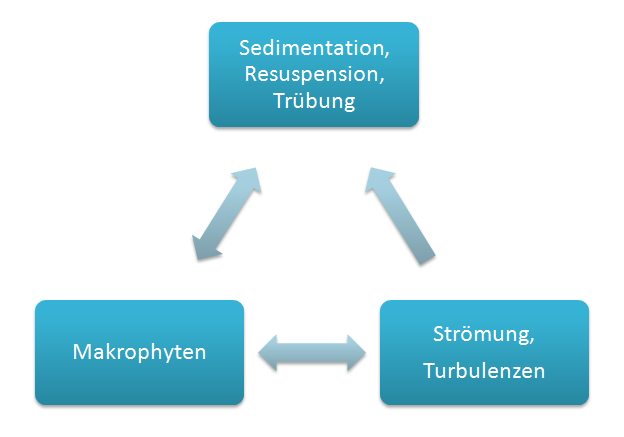
\includegraphics[width=0.68\textwidth]{images/Schema_Pfl_Sedim_Strm}
\caption[Zusammenhänge zwischen Makrophyten, Sediment- und Hydrodynamik]{Schematische Darstellung der komplexen Zusammenhänge zwischen Makrophyten, Sediment- und Hydrodynamik}
\label{fig:schema_Makrophyten,Sedimente,Hydrodynamik}
\end{figure}


Um festzustellen, ob es auch Unterschiede in den südlichen deutschen Boddengewässern in unterschiedlichen Vegetationsformen und -Wuchsdichten in bewachsenen und unbewachsenen Bereichen gibt, wurden an verschieden Stellen die Vegetation kartiert und das Sediment auf seine Korngrößenverteilung, den organischen Gehalt und den Wassergehalt hin untersucht.

Von besonderem Interesse war die Wechselwirkung zwischen Sediment und Wasser in einem bisher nur wenig und in diesem Zusammenhang überhaupt nicht untersuchten Ökosystem, dem Braunalgenbett aus Fucus vesiculosus f. balticus. Fucus vesiculosus, auch Blasentang genannt, ist eine in der Ostsee weit verbreitete Alge, deren Verschwinden jedoch, vermutlich aufgrund von Nähstoffbelastungen des Wassers und damit einhergehender reduzierter Sichttiefe und aufgrund von Änderungen des Salzgehaltes der Ostsee, seit 1976 beobachtet wird und deren Tiefengrenze sich in dieser Zeit von 10 auf etwa 4 Meter verlegt hat \citep{pehlke_2008}. 
Sie ist gelbbraun gefärbt und von derber Struktur, sitzt auf festem Gestein verankert und besitzt Gasblasen paarig an der Mittelrippe der Thallusäste angeordnet, die der photosynthesefähigen Zellfläche Auftrieb verleihen \citep{watermann_2013}.

Der Fucus vesiculosus f. balticus ist taxonomisch keine eigene Art, sondern stellt nach genetischen Untersuchungen lediglich eine Wuchsform von Fucus vesiculosus dar \citep{athanasiadis_1996}. Er siedelt auf Sand und schlickigem Sand in geschützten Buchten bis maximal \unit{2}{\metre} Tiefe \citep{{HELCOM}_2013} und ist nicht mit dem Untergrund verwachsen. Bei ausreichenden Bodenschubspannungen kann er verdriftet werden \citep{canal-verges_2010}.

Im Gegensatz zum festsitzenden Blasentang gibt es bisher keine veröffentlichten Studien, die den Einfluss des losen Blasentangs auf das Sediment untersuchen. Aufgrund seines Vorkommens auf Weichbodensubstraten in Flachwasserbereichen, stellenweise vergesellschaftet mit den typischen Brackwasser-Pflanzenarten wie Potamogeton pectinatus und Myriophyllum spicatum, kann man sagen, dass es sich um einen eigenständigen Biotoptyp handelt.\\
Der Habitus der Alge nimmt hier eine annähernd kugelförmige Gestalt an. Sie siedelt in einer hohen Dichte, wodurch der Wasseraustausch zwischen den Wasserschichten innerhalb des Algenbettes und darüber erschwert ist, sodass sich nach eigenen Beobachtungen von Mai bis Anfang Juni eine deutliche Thermokline feststellen ließ (in gleicher Wassertiefe ohne Fucus vesiculosus f. balticus wurde diese Thermokline nicht festgestellt). In diesem Zusammenhang wurde auch die Biomasse und ihr Einfluss auf das Sediment untersucht.

\cite{canal-verges_2010} fanden heraus, dass driftende Algen der Gattung Ulva sp., Ceramium sp. und Chaetomorpha linum die Resuspension erhöhen. Sie driften ab einer Strömungsgeschwindigkeit von \unit{2-3}{\centi\metre\per\second} über das Sediment und erodieren damit das Sediment. An Vergleichsstandorten ohne Algen hingegen begann die Resuspension erst ab einer Strömungsgeschwindigkeit von \unit{15-27}{\centi\metre\per\second}. Aus diesen Beobachtungen heraus ist es interressant zu untersuchen, ob dieses Phänomen auch auf die Algenmatte des baltischen Blasentanges zutrifft und sich demzufolge nicht viel feines organisches Material dort akkumuliert oder ob die phytale Decke so sehr in sich geschlossen ist und den Wasserkörper am Boden vor Strömung schützt, dass die Resuspension gemindert wird und das Sediment dadurch nicht feiner als an benachbarten unbedeckten Stellen ist.

Die Hypothesen, die im Zusammenhang mit den angeführten Erläuterungen auf die Anwendbarkeit in den Boddengewässern hin untersucht werden, sind folgende:


\begin{enumerate}[label=\Roman{*},leftmargin=1.5cm]

\item An Standorten mit dichter wurzelnder Vegetation ist der Anteil des organischen Materials im Sediment größer als an vegetationsarmen Standorten.

\item An Standorten mit einer dichten Bedeckung durch Makrophyten ist das Sediment feiner als an vegetationsarmen Standorten.  

\item Der Anteil der wurzelnden Pflanzen in der Wassersäule korreliert negativ mit der mittleren Korngrößenfraktion des Sedimentes.

\item An Standorten mit einer dichten Bedeckung durch Makrophyten ist das Sediment schlechter sortiert als an vegetationsarmen Standorten.

\item Die Sedimente an Stellen mit dichter Bedeckung durch Fucus vesiculosus f. balticus sind nicht feiner als an benachbarten Stellen ohne Vorkommen von Fucus vesiculosus f. balticus.

\item Der Organische Gehalt der Sedimente an Standorten mit dichter Bedeckung durch Fucus vesiculosus f. balticus ist nicht höher als an benachbarten Standorten ohne Fucus vesiculosus f. balticus. 

\item Die Sedimente werden im Verlauf der Vegetationsperiode mit dem Aufwachsen der Makrophyten feiner und ihr Anteil des organischen Gehalts erhöht sich.

\end{enumerate}


